\section{Compression Residuals}

\begin{figure}[h]
\centering
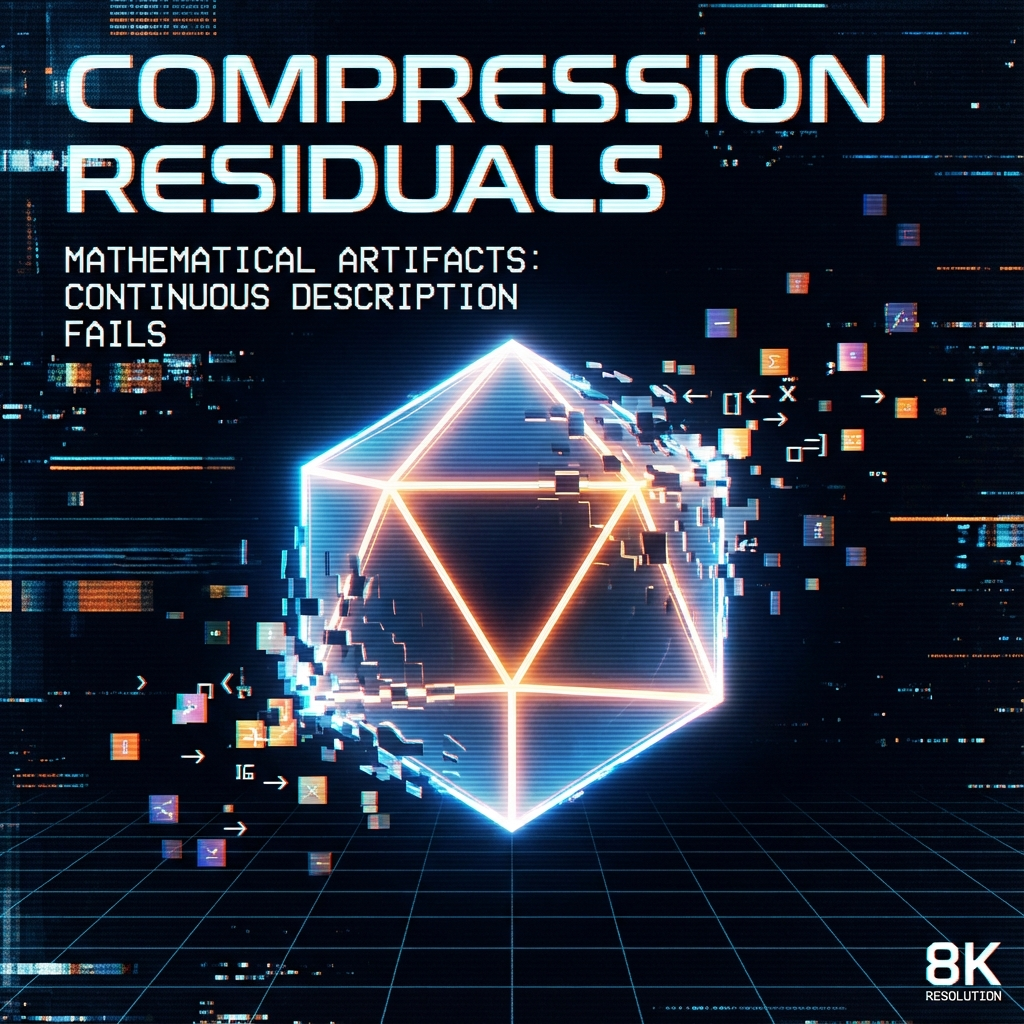
\includegraphics[width=0.8\textwidth]{assets/compression_residuals.png}
\caption{Compression Residuals}
\end{figure}

When we take a complex photo with a phone and save it as JPEG format, what happens? The phone's algorithm discards high-frequency details imperceptible to human eyes, approximating complex textures with smooth color blocks. This is \textbf{lossy compression}. Usually, this compression is very perfect. But if you photograph a black-and-white checkerboard image full of sharp edges and intense contrast, the compression algorithm collapses. At black-white boundaries, strange noise and artifacts appear.

These artifacts are not real objects; they are \textbf{residuals} (Residuals) inevitably produced when \textbf{describing discrete reality with smooth language}.

In our geometric reconstruction, modern physics---especially quantum field theory---plays exactly the role of that JPEG compression algorithm. And the particles in our eyes are those noise points.

\subsection{The Illusion of Continuity}

\begin{figure}[h]
\centering
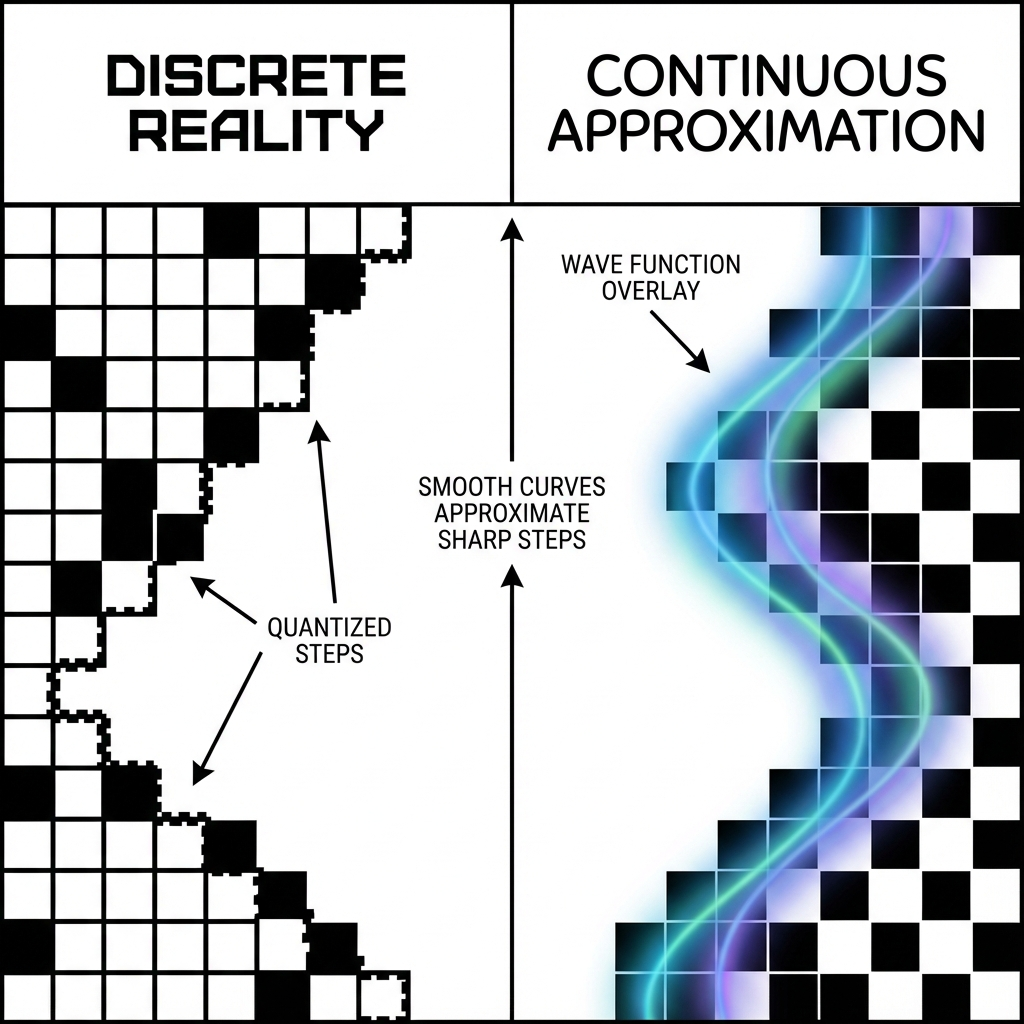
\includegraphics[width=0.8\textwidth]{assets/discrete_vs_continuous.png}
\caption{Discrete vs Continuous}
\end{figure}

As we showed in Chapter 6, the universe's foundation is likely a discrete Quantum Cellular Automaton (QCA) grid. But as macroscopic observers, our senses and instrument resolution are extremely limited. We cannot track every Planck pixel's jumping; we can only see their macroscopic average effects.

To describe these macroscopic effects, we invented \textbf{calculus}. We use continuous fields (Field) and smooth wave functions (Wavefunction) to approximate underlying discrete states.

In most empty cosmic space, this approximation is extremely perfect. Because grid state changes there are gentle, like blue sky in photos, smooth functions describe it perfectly. This is why vacuum appears so empty and smooth.

But when we encounter a \textbf{dead knot}---the topological defect mentioned in the previous section---trouble comes.

At the core of this dead knot, grid states undergo violent twisting and flipping. The change rate here is too fast; spatial structure too sharp. When we try to forcibly cover this region with smooth functions (continuous field theory), mathematical description fails.

To forcibly maintain the ``smooth'' illusion, our equations are forced to spit out an infinite value or an undefined singularity at this point. We circle this mathematically awkward point, label it, saying: ``There is a particle here.''

Therefore, \textbf{particles are lossy compression residuals of continuous field theory on discrete topological defects}.

\subsection{The Point Particle Paradox}

This view perfectly solves the ``point particle paradox'' that has plagued physics for a century.

In the standard model, electrons are described as geometric points with no volume. This leads to infinity disasters: if electrons were really just points, their charge density would be infinite, their self-energy also infinite. To escape these infinities, physicists had to invent complex ``renormalization'' techniques, essentially manually subtracting these infinities.

But from the QCA perspective, this is completely unnecessary trouble.

Electrons were never points. They are \textbf{topological knots with complex internal structure} at Planck scale. They occupy several grid points, have finite size, finite energy density.

The reason we write them as points in equations is that the ``continuous language'' we use has too low resolution to describe their exquisite internal pixel arrangement. We are forced to \textbf{compress} them into abstract points with no internal geometric structure, then have to additionally label these points with ``spin 1/2,'' ``charge -1'' to represent lost internal geometric information.

These quantum numbers (Quantum Numbers) are essentially \textbf{metadata of compression packages}. They are abbreviated encodings of those internal topological structures we cannot see.

\subsection{Not a Bug, but a Feature}

Programmers know that when code encounters unhandleable exceptions, the system throws an Error. In a sense, particles are \textbf{Errors} thrown by the universe operating system.

But this doesn't mean the universe is wrong. The universe runs perfectly fine. What's wrong is our \textbf{description method}.

\begin{itemize}
\item Universe ontology (QCA) is discrete, perfect, with no singularities.

\item Physical models (QFT) are continuous, approximate, full of singularities.
\end{itemize}

Particles behave so strangely---both wave-like and particle-like, both here and not here---precisely because they are caught between these two description systems. They are projections of discrete ghosts in the continuous world.

So when we talk about ``discovering new particles,'' we are not finding new building blocks in the universe's treasure box. We are exploring what new kinds of knots the underlying grid can tie. The Higgs boson (Higgs Boson) is not the God particle; it is a special vibration mode of the vacuum grid, a special compression residual.

This perspective liberates us from superstition about ``material entities.'' There are no ``things'' in the world; only \textbf{structures of information}.

Now, we know particles are dead knots on spatial structure. But since they are dead knots, why aren't they fixed? Why do they collide, bounce, even react?

This involves the second secret of ``time'' at the microscopic level: when time flows through these dead knots, it is no longer uniformly passing. It is drawn in, delayed, resonated.

This is the theme of our next chapter---\textbf{Time as Spectrum}. There, we will see how microscopic particles gain their dynamical behavior in the macroscopic world by ``devouring time.''

---

\textit{(Next, we will enter the final chapter of Part III---Chapter 8 ``Residence and Resonance,'' unraveling the temporal essence of microscopic interactions.)}

